% Chapter Template

\chapter{Test case} % Main chapter title

\label{case} % Change X to a consecutive number; for referencing this chapter elsewhere, use \ref{ChapterX}

\lhead{\emph{Test case}} % Change X to a consecutive number; this is for the header on each page - perhaps a shortened title

%----------------------------------------------------------------------------------------
%	SECTION 1
%----------------------------------------------------------------------------------------
\section{NASA Rotor 67 transonic axial compressor}

The test specimen for given analysis is a NASA Rotor 67 (R67) transonic axial compressor. Originating as a first stage of two stage fan for evaluation of design procedures, validation of experimental facilities as well as meshing and CFD tools. Both stages were used in a multitude of studies for aerodynamics, geometry optimisation, noise analyses and structural analyses. Full design procedure can be found in references \cite{r67design} and \citep{r67performance}. The CFD analysis and further post processing of the pressure signals shall be performed on a single passage of a first stage rotor of the compressor. The setup for the  calculations (apart from the single passage constraint) is relevant do case described in \citep{r67laser}, which was the main source for geometry and flowfield data.

\begin{figure}[h!]
\centering % bo \centering nie wstawia dodatkowego odstępu
\includegraphics[width=0.85\textwidth]{Pictures/r67_over.png}
\caption{Geometry of NASA R67}
\label{r67over}
\end{figure}

Basic figures of the given rotor are, design pressure ratio of 1.63 at massflow of 33.25 kg/sec. The design rotational speed is 16 043 rpm, which yields a tip speed of 429 m/s and an inlet tip relative Mach number of 1.38. The rotor has 22 blades and an aspect ratio of 1.56 (based on average span/root axial chord). The inlet and exit tip diameters are 514 and 485 mm, respectively, and the inlet and exit hub/tip radius ratios are 0.375 and 0.478, respectively. A fillet radius of 1.78 mm is used at the airfoil-hub juncture. The square root of the mean square of the airfoil surface finish is 0.8 $\mu${}m or better, the airfoil surface tolerance is $\pm$ 0.04 mm, and the running tip clearance is approximately 1.0 mm \citep{r67laser}. Surface roughness and some of the geometrical features are omitted during the preparation of the geometry and CFD mesh for reasons described in sections \ref{3dgeom} and \ref{mesh}. General geometry of NASA R67 is presented on fig \ref{r67over}


%-----------------------------------
%	SUBSECTION
%-----------------------------------
%\subsection{Efficiency figures}
%Nunc posuere quam at lectus tristique eu ultrices augue venenatis. Vestibulum ante ipsum primis in faucibus orci luctus et ultrices posuere cubilia Curae; Aliquam erat volutpat. Vivamus sodales tortor eget quam adipiscing in vulputate ante ullamcorper. Sed eros ante, lacinia et sollicitudin et, aliquam sit amet augue. In hac habitasse platea dictumst.

%-----------------------------------
%	SUBSECTION
%-----------------------------------
%\subsection{LDA Validation results}
%Morbi rutrum odio eget arcu adipiscing sodales. Aenean et purus a est pulvinar pellentesque. Cras in elit neque, quis varius elit. Phasellus fringilla, nibh eu tempus venenatis, dolor elit posuere quam, quis adipiscing urna leo nec orci. Sed nec nulla auctor odio aliquet consequat. Ut nec nulla in ante ullamcorper aliquam at sed dolor. Phasellus fermentum magna in augue gravida cursus. Cras sed pretium lorem. Pellentesque eget ornare odio. Proin accumsan, massa viverra cursus pharetra, ipsum nisi lobortis velit, a malesuada dolor lorem eu neque.

%----------------------------------------------------------------------------------------
%	SECTION
%----------------------------------------------------------------------------------------
\section{3D geometry preparation} \label{3dgeom}
Geometry was prepared in Ansys ICEM 14.5 meshing software. Creating the geometry directly in the meshing software reduces the risk of creating flaws in the geometry, due to file translations. Mesh is created in millimeters.

The R67 blade coordinates for rotor and stator on both stages is given in references \citep{r67design} and \citep{r67performance} and provide the blade elements in a Multiple-Circular-Arc fashion. In such approach the design blade elements lie on conical surfaces which approximate the actual stream flow surfaces. A blade-element-layout method is developed which preserves the constant-angle change characteristic of the circular-arc profile. More specifically, the mean camber line and the suction and pressure surface lines of a blade element are lines with a constant rate of angle change with path distance on a specified conical surface \citep{bladecompose}. Although relatively comfortable for design purposes, such approach requires implementing a macro or script to desired CAD tool for creating the blade elements or transforming the MCA blade to Cartesian or cylindrical coordinates. Reference \citep{bladecompose} provides an extended definition of MCA blade description as well as Fortran code for generating blade cross-section and geometric properties of the blade. Source \citep{r67laser} provides a list of coordinates for 14 profiles of the 1st stage rotor blade suction and pressure side, as well as coordinates for hub and casing int the meridional plane. These coordinates were used to create the geometry of the single passage of the subject blade. Coordinates are also available in Appendix \ref{r67_coords_data} and project Github repository \citep{github}.

%Geometry alignment is presented on figure \ref{geom_gcs}.
The coordinate system is a standard right-hand Cartesian CS. Rotation axis is set to Z-axis with flow in positive Z direction. The compressor rotation is set as in right-hand rule, the compressor rotates in clockwise direction when facing the blade leading edge. $Z = 0$ coordinate is defined by point number 1 on 1st blade design surface (see Appendix \ref{r67_coords_data} for details). 

%\begin{figure}[h!]
%\centering % bo \centering nie wstawia dodatkowego odstępu
%\includegraphics[width=0.85\textwidth]{Pictures/kitten-placeholder.jpg}
%\caption{Global coordinate system for geometry}
%\label{geom_gcs}
%\end{figure}

Hub and casing flow path were created by importing formatted point data as a b-spline curve, followed by extrusion the curve to surface by rotating it by $\pm 60 \degree$. Blade surfaces cylindrical coordinates were transformed to Cartesian coordinates using simple trigonometric calculations and imported as set of splines. Suction and pressure surface of the blade were created by lofting the surface along the imported splines. Leading and trailing edge radii were created in a similar manner with use of edge radius and edge tangency points given in \citep{r67laser}. Tip gap of the blade was created by offsetting the casing surface by 1.016 mm in the normal direction towards the rotation axis and creating a section line between blade surfaces and the offset surface.

Due to the estimated mesh cell count, only one blade passage is created, therefore a set of periodic surfaces must be defined. ICEM software is capable of creating a midline as an average of coordinates of two given lines. A midline was created for every design profile and was manually extended beyond the blade leading and trailing edge. Midlines were lofted to create a midsurface which was later on copied with rotation by $\pm 0.5 \cdot \frac{360 \degree}{22}$ to create two identical periodic surfaces.

Aforementioned midlines were also rotated along Z-axis to create control surfaces for mesh stabilization and data acquisition down the process.

Reference \citep{r67laser} provides coordinates of hub and casing for the full experiment, however only a rotating part of the experimental rotor setup will be used. Two surfaces normal to Z direction at coordinates Z = -13.74 mm and Z = 93.65 mm are placed as inlet and outlet boundary conditions. Geometry was finished by necessary extrusions, trimming and other finishing operations to ensure high quality surface for meshing. Usually, the geometry must be watertight  to ensure proper meshing process, however ICEM as patch-independent meshing software does not require that.

Physical experiment test compressor has a 1.78 mm fillet at airfoil-hub juncture. This feature was omitted as it would unnecessarily complicate the meshing process and increase the cell count.

Such approach allowed for creating a geometry for single blade passage with centered blade of 1st stage rotor of the test compressor (Fig \ref{geom_final}).

\begin{figure}[ht!]
\centering % bo \centering nie wstawia dodatkowego odstępu
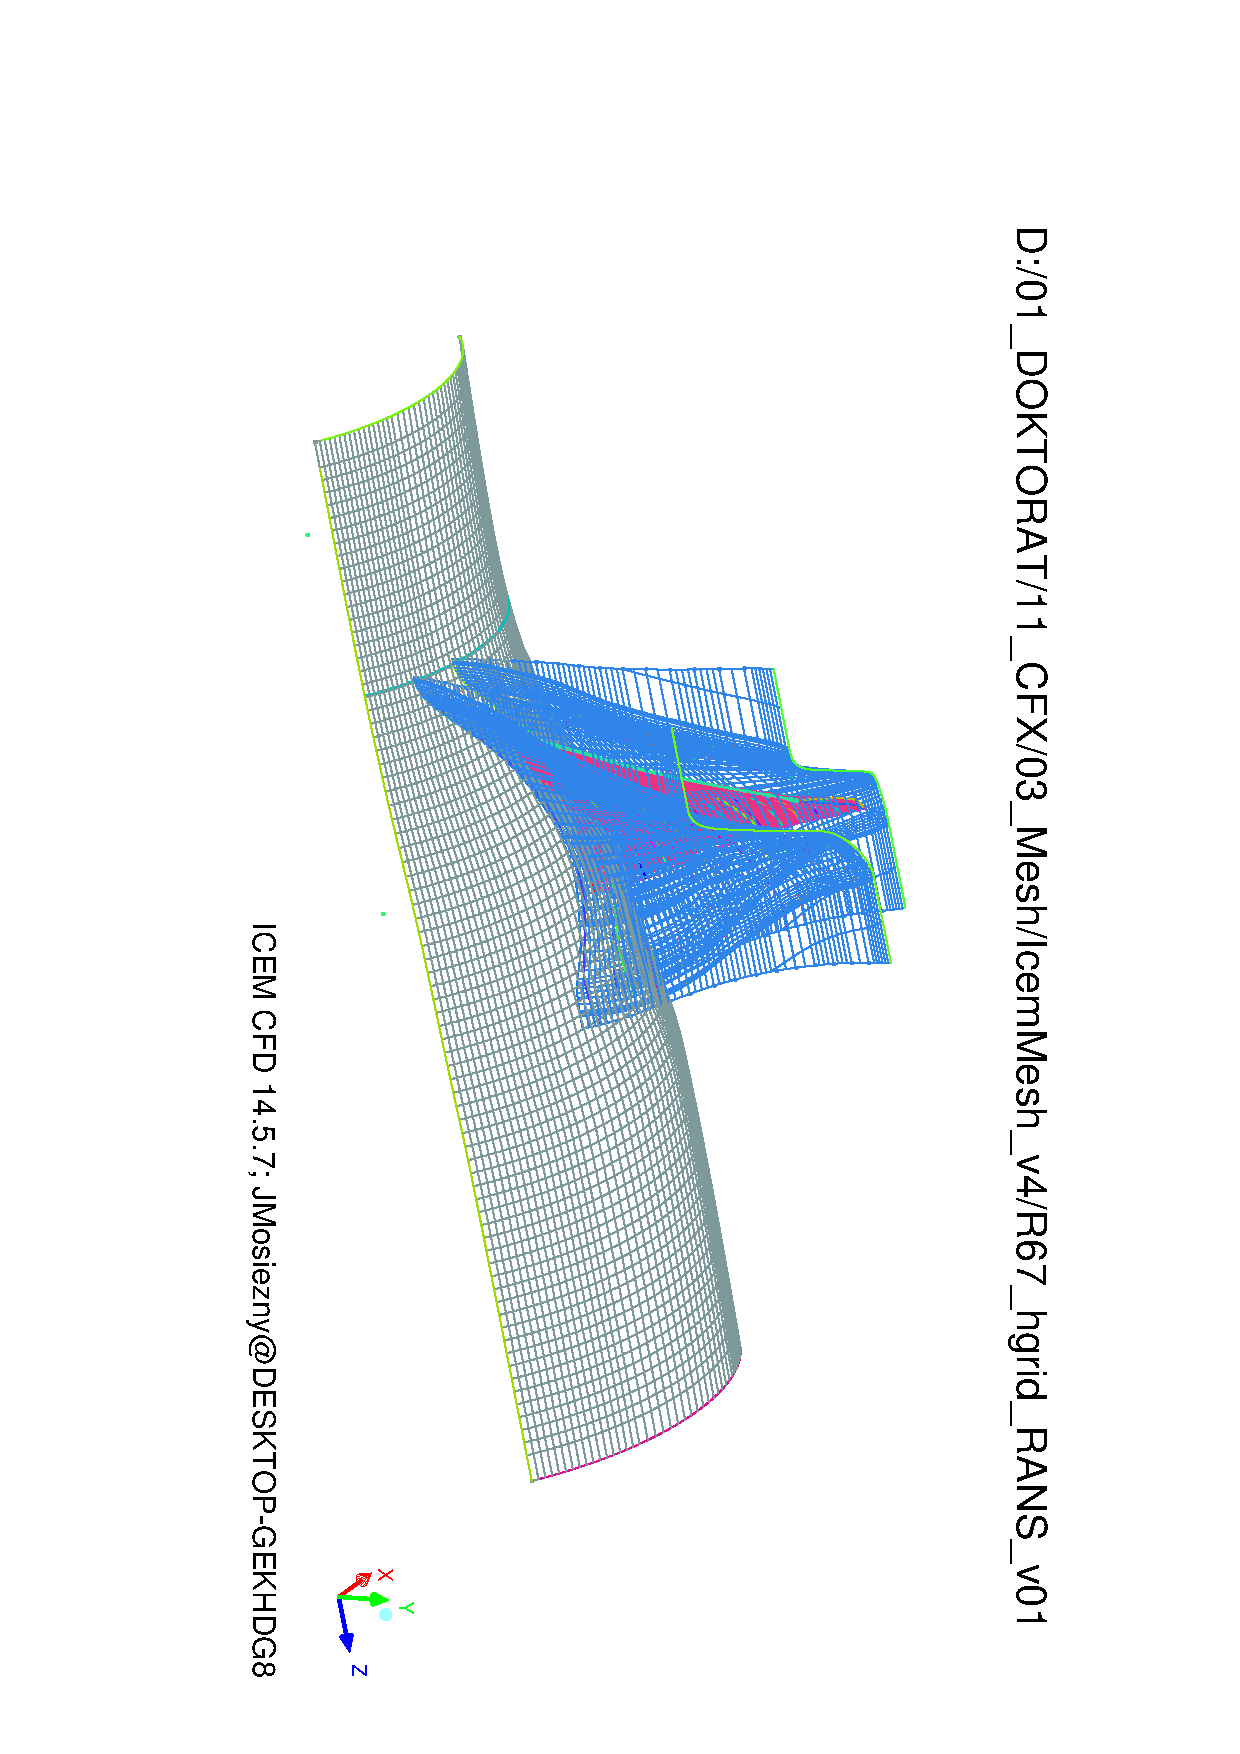
\includegraphics[width=0.85\textwidth]{Pictures/r67_geom.jpg}
\caption{Final single passage geometry. Some features hidden for clarity}
\label{geom_final}
\end{figure}

%----------------------------------------------------------------------------------------
%	SECTION
%----------------------------------------------------------------------------------------
\section{Meshing approach} \label{mesh}
Following requisites are posed to the mesh for the discussed case:
\begin{itemize}
\item Possibly low number of elements fulfilling the mesh sizing requirements stated in chapter \ref{direct_approach},
\item Mesh should be a fully structural mesh including the tip gap,
\item The periodic boundary mesh must be identical/conforming for both boundaries,
\item The mesh must have high quality metrics in terms of cell orthogonality and skew as defined by equations \ref{eq:ortho} \& \ref{eq:skew} respectively.
%\item The cell aspect ratio should be limited to 5000 as defined by equation \ref{eq:aspect} 
\end{itemize}


\begin{equation} \label{eq:ortho}
\text{Orthogonality} = \frac{\vec{A_i} \cdot \vec{f_i}}{|\vec{A_i}| \cdot |\vec{f_i}|}
\end{equation}


\begin{equation} \label{eq:skew}
\text{Skewness} = \frac{\text{Optimal Cell Size} - \text{Cell Size}}{\text{Optimal Cell Size}}
\end{equation}

%\begin{equation} \label{eq:aspect}
%Aspect Ratio = \frac{MinimumElementEdge}{MaximumElementEdge}
%\end{equation}

One of the initial mesh concepts was an unstructured mesh with triangular surface mesh extruded to prism boundary layer and mostly isotropic tetrahedra in the volume. This approach was quickly rejected for bad quality elements near the airfoil/hub junction and tip gap, as well as element count in range of 4.5 million cells for sizing relevant for RANS analysis. This approach was quickly dropped.

A non-trivial topology with fully conforming periodic boundaries was introduced (fig \ref{cj_topo}). This topology fulfills all the prerequisites stated apart from possibility to mesh a structural tip gap. Such approach makes it impossible from topological standpoint to place a structural mesh in this area. A RANS sufficient mesh without tip gap area (blade was extended to the casing surface) was created. The cell count for this mesh is below 0.5 million cells with better skewness and orthogonal quality. This mesh was utilized for numerical setup and data acquisition testing as it was faster to converge.

\begin{figure}[h!]
\centering % bo \centering nie wstawia dodatkowego odstępu
\includegraphics[width=0.85\textwidth]{Pictures/r67_cj.jpg}
\caption{Mesh topology with conforming periodic boundaries}
\label{cj_topo}
\end{figure}

Final topology was a standard h-grid topology for airfoil \ref{h_topo}. Although it is impossible to create a conforming periodic interface with such mesh topology, a fully structural tip gap was implemented. Omitting the blade-hub juncture fillet simplified the mesh.  Such topology eradicates the necessity of placing 5-way topology points.

\begin{figure}[h!]
\centering % bo \centering nie wstawia dodatkowego odstępu
\includegraphics[width=0.85\textwidth]{Pictures/r67_htopo.jpg}
\caption{Mesh h-topology}
\label{h_topo}
\end{figure}

Mesh was created in Ansys ICEM software using structural blocking method. The topology was sliced and associated to internal surfaces mentioned in the above section. This enforces mesh layering along design streamlines and provides high quality mesh on internal surfaces for flow field data acquisition further in the process. Blade wall boundary condition is distributed among five separate parts: blade pressure side, blade suction side, leading and trailing edges and tip surface. 

Element sizing in volume and in tangent direction to the blade is limited to 3 mm, with 5 mm at inlet and outlet boundary conditions. The mesh sizing requirements are described in chapter \ref{approach}.  Blade boundary layer is produced by creating an o-grid around blade geometry. Hub and casing boundary layers are created by changing the sizing on the blocks adjacent to the geometry. Sizing of the first element is estimated with y+ parameter as described in equation: \ref{eq:yplus}. First element thickness in on the blade surfaces ranges from is $2 \mu m$ on tip airfoil and $10 \mu m$ on hub airfoil. This corresponds to $y^{+} \approx 2$ calculated by streamline velocity values given in \citep{r67laser}.

\begin{equation} \label{eq:yplus}
\Delta s = \frac{y^{+} \mu}{U_{fric} \rho}
\end{equation}

Where:
\begin{equation}
U_{fric} = \sqrt{\frac{\tau_{wall}}{\rho}}
\end{equation}

Where:
\begin{equation}
\tau_{wall} = \frac{C_f \rho U_{\infty}^{2}}{2}
\end{equation}

Where:
\begin{equation}
C_f = \frac{0.026}{Re_{x}^{1/7}}
\end{equation}

Internal volume of the mesh was stabilized by attaching the mesh blocks to the internal design surfaces. This ensures that mesh layers are mostly coincident with the primary compressor flow. The internal surface mesh is also used as an internal boundary marker for data acquisition purposes. The markers are named \texttt{hub}, \texttt{int-01} thru \texttt{int-12} and \texttt{int-tip} corresponding to following locations of the design surfaces.

\begin{table}[htb!]
\centering
\caption{Location of compressor desing surfaces} \label{tab:surfs}
\begin{tabular}{ | l | r | } \hline
Boundary marker & Location \\ \hline \hline
\texttt{hub} & 0\% span  \\ \hline
\texttt{int-01} --- \texttt{int-12} & 7.7\% --- 92.3\% every 7.7\% span \\ \hline
\texttt{int-tip} & 100\% span \\ \hline
\end{tabular}
\end{table}

Figure \ref{mesh-ortho}, provides overview of mesh quality defined by figure \ref{eq:ortho}. Created mesh is of high quality and is sufficient for both RANS and DDES analyses (chapter \ref{cfd}). Final mesh reached roughly 11.5 million cell count. Final mesh is presented in figure \ref{meshfinal} 

\begin{figure}[h!]
\centering % bo \centering nie wstawia dodatkowego odstępu
\includegraphics[width=0.85\textwidth]{Pictures/mesh_ortho.png}
\caption{Mesh non-orthogonality histogram}
\label{mesh-ortho}
\end{figure}

\begin{figure}[h!]
\centering % bo \centering nie wstawia dodatkowego odstępu
\includegraphics[width=0.85\textwidth]{Pictures/r67_ransmesh.jpg}
\caption{Completed Mesh}
\label{meshfinal}
\end{figure}

%----------------------------------------------------------------------------------------
%	SECTION
%----------------------------------------------------------------------------------------
%\section{Data acquisition} \label{casedata}
%Mesh and case is set up for possibly efficient data acquisition of flow field pressure and velocity data. FLUENT data file from a single timestep takes around 2GB of disk space. Saving such dataset from every of 50150 timesteps requires about 97TB of storage, which was unavailable at the time. 
%
%Data was gathered from blade surface (5 boundary markers) and 13 internal markers. Following node data values were saved:
%
%\begin{itemize}
%\item Static pressure
%\item Velocity magnitude (only internal markers)
%\item Vorticity magnitude (only internal markers)
%\item Static density
%\item Static temperature
%\item Node coordinates
%\end{itemize}
%
%This approach generated 18 datasets of 50510 files each, resulting in taking up 5.5TB of HPC cluster storage. The number of data is still large but manageable with current software engineering tools. Data was saved to ASCII text files.